%!TEX root = TFG.tex

\chapter{Estado del arte}

En este capítulo se realiza un estudio del estado del arte relativo a la aplicación de distintas técnicas que tengan como objetivo identificar a un dispositivo a través de la red independientemente de un identificador susceptible de ser identificado. Para estos cometidos son muy utilizados los algoritmos de aprendizaje automático o Machine Learning. 

Comenzamos la revisión bibliográfica por el trabajo desarrollado por Pascal Oser et al. \cite{oser2018identifying}. En este trabajo se desarrolla un sistema para identificar dispositivos entre un total de 562 en el centro del CERN. Para este cometido se tomas muestras periódicas de las marcas de tiempo (timestamps) contenidas en paquetes TCP que se envían y reciben de estos dispositivos.

De estas marcas se obtienen las variables que se usarán para entrenar los distintos modelos de machine learning. Las variables que obtiene son el incremento entre dos marcas consecutivas, el desbordamiento del contador de la marca de tiempo, la mediana de todas las marcas, etc.

Una variable interesante es la del desbordamiento del contador. En el RFC 1323 \cite{RFC1323} se define que el contador del timestamp (campo TSval) tiene una longitud de 4 bytes (32 bits), por lo tanto, el mayor valor que podrá tener asignado es $2^{32}$, puesto que es un entero sin signo. Se podría pensar que todos los dispositivos desbordan a la vez, pero cada fabricante establece el valor al que el contador se desborda. Esto está ilustrado en la Fig. \ref{fig:cern_ts_overflow} con dos ejemplos.

\begin{figure}
    \centering
    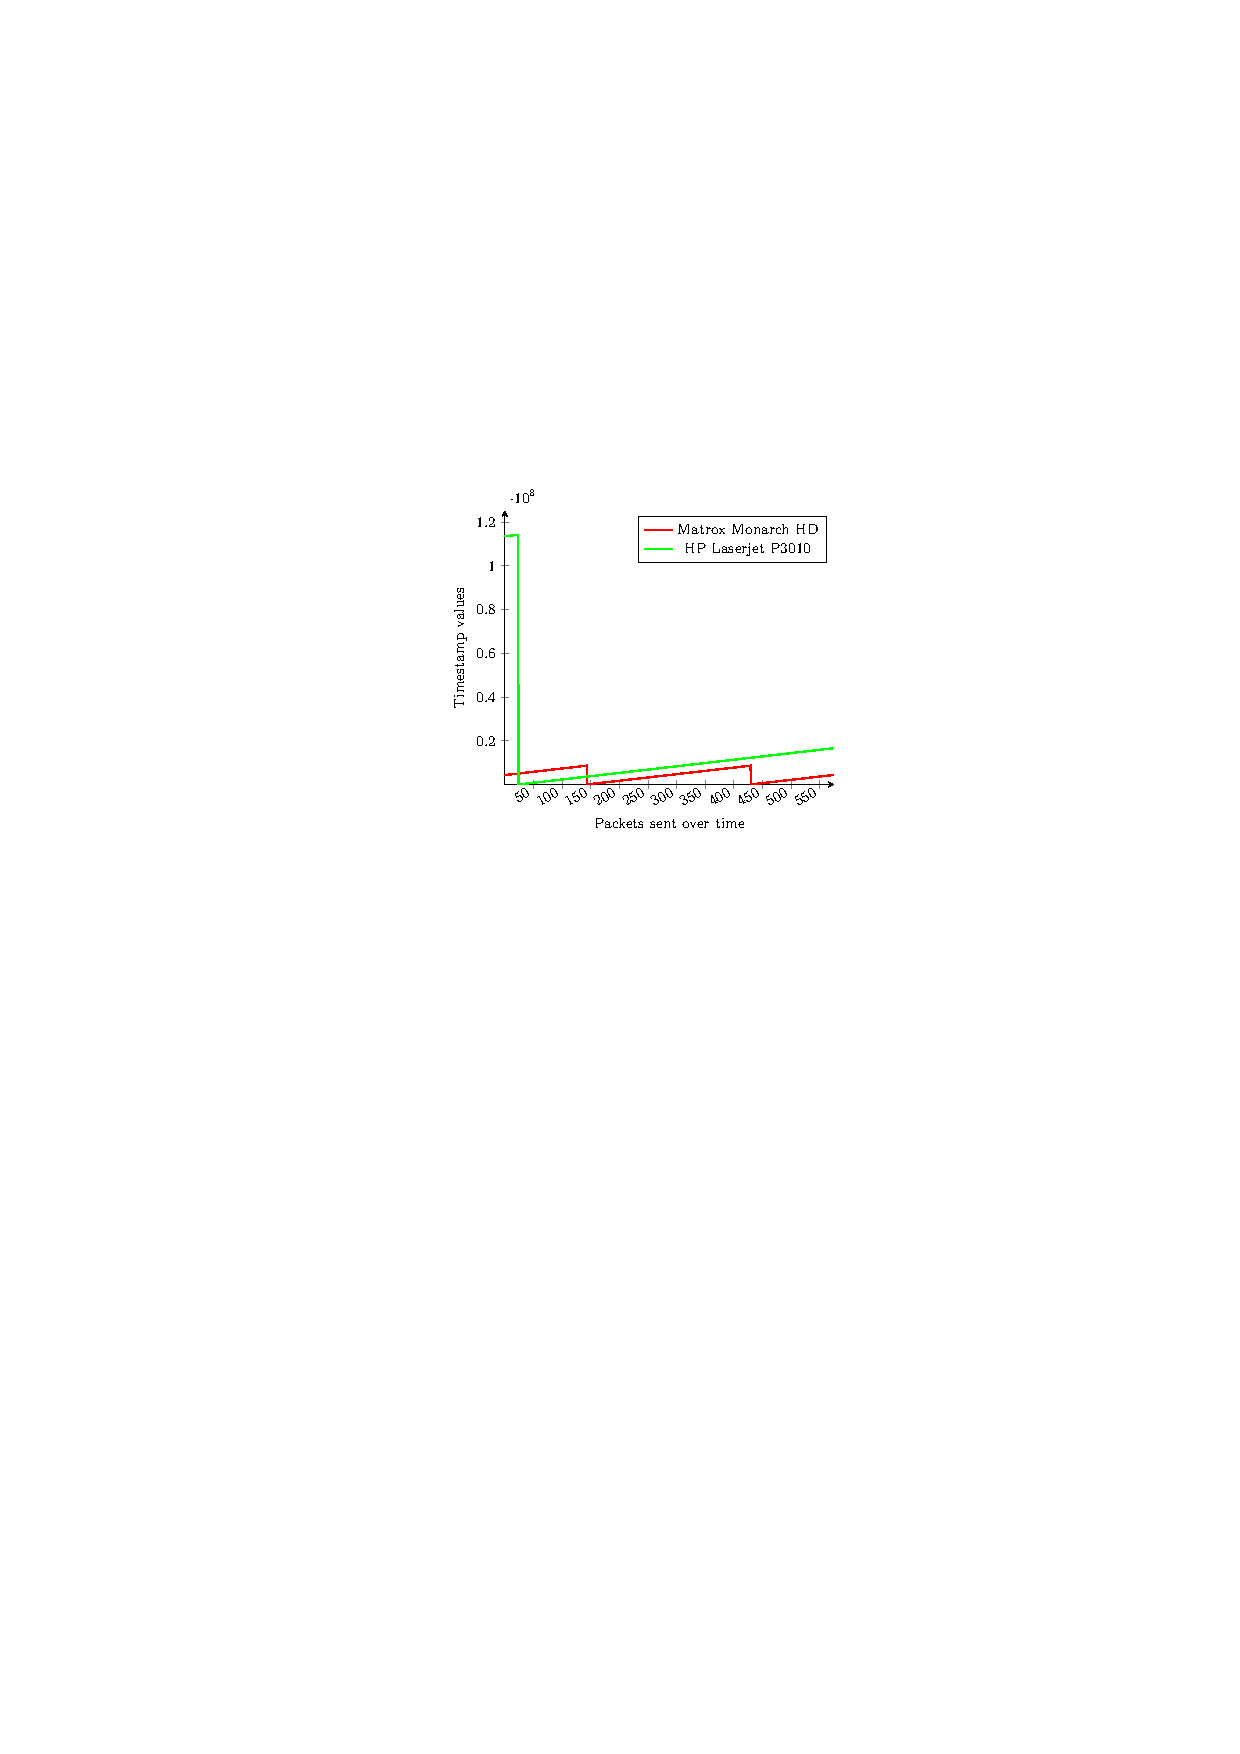
\includegraphics[width=0.45\textwidth]{images/CERN-timestamp_overflow}
    \caption{Desbordamiento del contador \cite{oser2018identifying}}
    \label{fig:cern_ts_overflow}
\end{figure}

Una vez tiene todas las variables registradas para todos los dispositivos, compara varios modelos de machine learning, para clasificar cada uno de los dispositivos. Los resultados que obtiene son de un accuracy del 99.22\% con MLP, un 99.14\% con SVM y por último 99.67\% con Random Forest.

Con estos datos decide quedarse con el modelo de Random Forest, el cual entrena con la totalidad de los datos de entrenamiento, obteniendo finalmente una precisión del 97.03\% y un accuracy del 99.76\%.

Otro trabajo relacionado con la temática ha sido desarrollado por Salma Abdalla Hamad et al. \cite{hamad2019iot}. En este trabajo se desarrolla un sistema que identifique a un dispositivo que quiere conectarse a la red y decida si se le permite realizar esta acción o se le deniega. Además este sistema comprobará periódicamente los dispositivos que están ya en la red para detectar comportamientos malintencionados. 

Este sistema (Fig. \ref{fig:diam_hamad}), una vez se tiene una traza del dispositivo que se quiere conectar por primera vez a la red, crea una huella del dispositivo que será analizada por un modelo (previamente entrenado) que lo clasificará como desconocido o no, en caso de que esté en una lista blanca. En caso de ser un dispositivo desconocido se le denegará el acceso a la red. Por contra, si está en la lista, se consultará una matriz de autorización (que contiene la confianza de ese dispositivo según sus vulnerabilidades) para saber que privilegios recibirá ese dispositivo. Con esto el dispositivo puede contectarse como un dispositivo ``confiable'', teniendo acceso a comunicarse con todos los dispositivos de la red, o por contra, de ``acceso restringido'' donde solo podrá comunicarse con dispositivos de ese mismo nivel de acceso.

\begin{figure}
    \centering
    \resizebox{0.6\textwidth}{!}{
        \begin{tikzpicture}
    \node[draw, text width = 2cm, align = center, minimum width = 2cm, fill = blancodiagrama, execute at begin node=\setlength{\baselineskip}{1em}] (1) {\footnotesize Sequence Capture};
    \node (2) [left = 3cm of 1] {};
    \node[draw, rounded corners, fill = azuldiagrama] (3) [below = of 1] {\footnotesize Finger Print};
    \node[draw, diamond, aspect = 2, fill = azuldiagrama] (4) [below = of 3] {\footnotesize Classifier};
    \node[draw, cylinder, rotate = 90, fill = verdediagrama, minimum height = 0.5cm, minimum width = 0.5cm, scale = 0.5] (5) at (-0.9,-3.85) {};
    \node[draw, rounded corners, fill = azuldiagrama] (6) [below = of 4] {\footnotesize Zoning};
    \node (7) [left = 3cm of 6] {};
    \node (8) [below = of 6] {};
    \node[draw, fill = verdediagrama] (9) [left = of 8] {\footnotesize Trusted};
    \node[draw, fill = naranjadiagrama] (10) [right = of 8] {\footnotesize Restricted};
    \node[draw, text width = 2cm, align = center, minimum width = 2cm, fill = blancodiagrama, execute at begin node=\setlength{\baselineskip}{1em}] (11) [below = of 8] {\footnotesize Random Capture};
    \node[draw, rounded corners, fill = azuldiagrama] (12) [below = of 11] {\footnotesize Finger Print};
    \node[draw, diamond, aspect = 2, fill = azuldiagrama] (13) [below = of 12] {\footnotesize Classifier};
    \node[draw, cylinder, rotate = 90, fill = verdediagrama, minimum height = 0.5cm, minimum width = 0.5cm, scale = 0.5] (14) at (-0.9,-12.73) {};
    \node[draw, ellipse, minimum height = 1.5cm, fill = verdediagrama] (15) [left = of 13] {\footnotesize Match};
    \node[draw, fill = rojodiagrama] (16) [left = 2.5cm of 9] {\footnotesize Rejected};
    \node[draw, fill = rojodiagrama] (17) [right = 2.5cm of 10] {\footnotesize Quarantine};
    \node (18) [above right = 4.7cm of 13] {};
    \node (19) [below right = 0.7cm of 13] {};
    
    \draw (2) -- (1) node [midway, above, text width = 2.5cm, align = center] {\footnotesize Unseen Device Network Traces};
    \draw (2) -- (1) node [midway, below, text width = 2.5cm, align = center] {\footnotesize 010111000011001};
    \draw (1) -- (3);
    \draw (3) -- (4);
    \draw (4.west) -| (16.north) node [pos=0.25, above] {\footnotesize Unknown Device};
    \draw (4) -- (6);
    \draw (7) -- (6) node [above, midway] {\scriptsize Authorisation Matrix};
    \draw (6) -- (9);
    \draw (6) -- (10);
    \draw (9) -- (11);
    \draw (10) -- (11);
    \draw (11) -- (12);
    \draw (12) -- (13);
    \draw (15) -- (13);
    \draw (13) -| (18.center) node [pos=0.25, above] {\footnotesize Mis-Classified} |- (6);
    \draw (13) |- (19.center) -| (17) node [pos=0.17, above] {\footnotesize Suspicious/Mis-Behaving};
\end{tikzpicture}
    }
    \caption{Modelo del sistema de identificación \cite{hamad2019iot}}
    \label{fig:diam_hamad}
\end{figure}

Para los dispositivos que ya están conectados a la red, se toma una muestra aleatoria que comprobará si se han clasificado de forma correcta. En el caso de que se haya clasificado mal pero siga estando en la lista blanca se actualizará su matriz de autorización. Por otra parte, en caso de que no esté en dicha lista se pondrá en cuarentena para ser analizado más adelante.

Las huellas de los dispositivos se obtienen del payload de los mensajes enviados por ese dispositivo. De ellos se obtienen 67 características como el tamaño del paquete Ethernet, el tamaño de las cabeceras, la IP de destino, el TTL, etc.

Con estas huellas entrena distintos modelos como son AdaBoost, LDA, KNN, Árboles de decisión, Naive Bayes, SVM, Random Forest y GBoost. Obtuvo un accuracy final del 89\%.

El siguiente artículo que se analizará es el realizado por Ahmet Aksoy et al. \cite{aksoy2019automated}. Este trabajo diseña un sistema (llamado SysID) que es capaz de identificar dispositivos a través del tráfico de red. 

Este sistema únicamente necesita un paquete de red para identificar el dispositivo. Dado un paquete de la traza se seleccionan $n$ cabeceras del paquete mediante un algoritmo genético, que implementa una función fitness (Eq. \ref{eq:aksoy_fit}) que trata de reducir este número de cabeceras. 

\begin{equation}
    Fitness = 0.9 \cdot Accuracy + 0.1 \cdot \left( 1 - \frac{\lvert SelectedFeatures \rvert - 1}{\lvert AllFeatures \rvert - 1} \right)
    \label{eq:aksoy_fit}
\end{equation}
donde $n = \lvert SelectedFeatures \rvert$ y $Accuracy$ es el resultado que se obtiene del modelo de machine learning entrenado con esas cabeceras.

Las trazas que se han usado para clasificar estos dispositivos provienen de una base de datos de otro artículo \cite{miettinen2017iot}, de donde se obtienen 20 medidas de 23 dispositivos IoT.

Para la clasificación se han usado diferentes algoritmos de la herramienta WEKA \cite{hall2009weka} como son tablas de decisión, árboles de decisión J48, OneR y PART. Se decide usar una clasificación en dos niveles (Fig. \ref{fig:askoy_classifier}), se clasifican primero entre su proveedor o el propio dispositivo, dependiendo de si hay más de un mismo dispositivo del mismo proveedor. Después se clasifican los dispositivos del mismo proveedor entre sí. Este esquema ayuda a tener mejores resultados pues cada proveedor puede ser identificado de mejor forma por un algoritmo distinto.

Los resultados que obtiene son de un 82\% de accuracy promedio entre todos los clasificadores de cada proveedor. Los valores individuales están entre el 42.2\% y el 100\%.

\begin{figure}
    \centering
    \resizebox{0.6\textwidth}{!}{
        \begin{tikzpicture}
    \node[draw, fill = azulclasificador, minimum width = 4.5cm] (0) {Hue Classifier};
    \node[draw, fill = azulclasificador, minimum width = 4.5cm] (1) [left = of 0] {Device Genre Classifier};
    \node[draw, fill = azulclasificador, minimum width = 4.5cm] (2) [above = 0.4cm of 0] {EdimaxPlug Classifier};
    \node[draw, fill = azulclasificador, minimum width = 4.5cm] (3) [above = 0.4cm of 2] {D-Link Classifier};
    \node[draw, fill = azulclasificador, minimum width = 4.5cm] (4) [below = 0.4cm of 0] {TP-Link Classifier};
    \node[draw, fill = azulclasificador, minimum width = 4.5cm] (5) [below = 0.4cm of 4] {Smarter Classifier};
    \node[draw, diamond, shape aspect = 2, fill = rojoclasificador] (6) [below = 0.4cm of 5] {Result};
    \node[draw, diamond, shape aspect = 2, fill = rojoclasificador] (7) [right = of 0] {Result};
    \node[draw, tape, tape bend top = none, tape bend height = 6pt, text width = 2.3cm, align = center, fill = verdeclasificador] (8) [above = 1.72cm of 1.west, anchor = west] {Arff file \\ (All devices)};
    
    \draw (1) -- (0);
    \draw (1.north) to [bend left = 18] (2.west);
    \draw (1.north) to [bend left] (3.west);
    \draw (1.south) to [bend right = 18] (4.west);
    \draw (1.south) to [bend right] (5.west);
    \draw (1.south) to [bend right] (6.west);
    
    \draw (0) -- (7);
    \draw (3.east) to [bend left] (7.north); 
    \draw (2.east) to [bend left] (7.north west); 
    \draw (4.east) to [bend right] (7.south west); 
    \draw (5.east) to [bend right] (7.south); 
    
    \draw (8) -- (8 |- 1.north);
\end{tikzpicture}
    }
    \caption{Clasificador de dos niveles \cite{aksoy2019automated}}
    \label{fig:askoy_classifier}
\end{figure}

El siguiente trabajo que se verá es el realizado por Hossein Jafari et al. \cite{jafari2018iot}. En este artículo no se utilizan paquetes de la capa de red o transporte, sino de la capa física. Para realizar esta labor se obtendrá la huella de cada dispositivo mediante radio frecuencias, por esta razón, este estudio sólo se centrará en conexiones inalámbricas, en este caso 6 dispositivos ZigBee.

Para cada uno de los dispositivos se realiza una captura de 5 minutos. Esta captura será del SNR en 5 niveles distintos, con lo que se obtiene \SI{10}{\giga\byte} por dispositivo y nivel de SNR, lo que en total serían \SI{300}{\giga\byte} de datos.

A continuación procede a entrenar tres modelos de deep learning, DNN, CNN y LSTM (los tres modelos pertenecen a la librería \texttt{TensorFlow} programada para Python \cite{tensorflow2015-whitepaper}), con los que obtiene unos resultados de 96.3\%, 94.7\% y 76\% respectivamente.

Por último realizaremos un resumen en forma de tabla de los artículos que han sido revisados.

\begin{table}[H]
    \centering
    \begin{tabularx}{0.9\textwidth}{Y|Y|Y}
        Propuesta & Algoritmos usados & Resultados \\
        \hline\hline
        Pascal Oser et al. \cite{oser2018identifying} & MLP, SVM, Random Forest & 99.76\% de accuracy y 97.03\% de precisión \\
        \hline
        Salma Hamad et al. \cite{hamad2019iot} & AdaBoost, LDA, KNN, Árboles de decisión, Naive Bayes, SVM, Random Forest y GBoost & 89\% de accuracy \\
        \hline
        Ahmet Aksoy et al. \cite{aksoy2019automated} & Tablas de decisión, Árboles de decisión J48, OneR y PART & Entre 42.2\% y 100\% de accuracy, con un promedio de 82\% \\
        \hline
        Hossein Jafari et al. \cite{jafari2018iot} & DNN, CNN y LSTM & 96.3\% de accuracy en DNN, 94.7\% de accuracy en CNN y 76\% de accuracy en LSTM
    \end{tabularx}
    \caption{Resultados en el estado del arte}
    \label{tab:art_results}
\end{table}


